\documentclass[../HFT-main.tex]{subfiles}
%\usepackage{cleveref}

%% --- Hyperref settings ---
%\hypersetup{
%  colorlinks=true,
%  linkcolor=black,
%  citecolor=black,
%  urlcolor=blue
%}

%% --- IEEE biblatex setup w/ url citations--- %%% Same header as CASE.tex. But doesn't work
%\usepackage[
%  backend=biber,
%  style=ieee,
%  url=false,
%  doi=false,
%  isbn=false
%]{biblatex}
%\addbibresource{../../REFERENCES/MASTER_REFERENCES.bib}

\title{Principles of Operation}

\begin{document}

\clearpage

\begin{marginfigure}	% Trim is left, bottom, right, top
\centering
   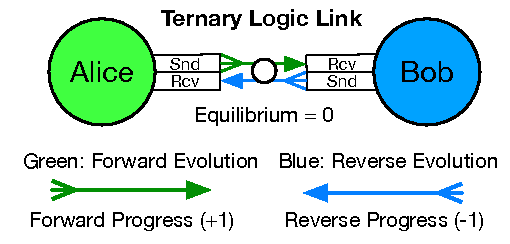
\includegraphics[width=1.15\textwidth]{../figures/ternary-link.pdf}
\caption{\centering Two \texttt{CELLs} and a \LINK with \emph{Conserved Quantities} (CQ) in dynamic equilibrium (Alternating Bit Protocol), epistricted with \href{https://en.wikipedia.org/wiki/Three-valued_logic}{Ternary Logic}}% \cite{threevaluedlogic2025}}
\label{fig:LINK}
\end{marginfigure}

\section{\Huge Principles of Operation}

\subsection{Symmetric Reversibility}

This protocol is  \texttt{symmetric} and \texttt{reversible}.  Asymmetry occurs  when one party becomes the \texttt{INITIATOR}, and the other party becomes the \texttt{RESPONDER}. When the responder is complete and closes the transaction with the sender, the \LINK returns to the equilibrium state. There is no need for counting protocols. Accounting of Shannon information is \emph{how far we deviate from equilibrium}, and what precisely is needed to bring it back.

\subsection{Atomicity and Causal Determinism}

\marginnote{To begin and remain \emph{open}, this protocol is based on the earliest known prior art  [Bartlett, Lynch \& Metcalfe]}% \cite{Bartlett1969,Lynch1968,metcalfe_ethernet_1976}}
%(IP in public domain)

Causal \texttt{operators} follow a mathematical framework of invertibility and an equilibrium state (\S). Equilibrium is maintained in the \LINK through continually circulating  tokens in the PHI layer, to maintain \texttt{liveness}, keeping  \LINKs in a state of preparedness for  transactions.  \marginnote{This mathematical symmetry is reflected throughout the architecture RISC-like radical minimalist design.}  

\subsection{Shift from promiscuous Bandwidth "rate" to causal Interaction "rate"}

Initiators Flow Frames (without stopping), to responders. Responders flow responses (without stopping) back to initiators. 

\subsection{Race Conditions and Conserved Quantities}

\marginnote{For short-range  $\le1m$ links,  intrinsic (internal ASIC or FPGA) \emph{rates} of the SerDes dominate, making cable propagation `time' and RTT irrelevant because the occupation length of the packet exceeds the length of the wire. \\With appropriate buffering and pipeline management, maximum Ethernet throughput becomes achievable, strongly favoring short-range interconnects for high-performance and ultra- low-latency Ethernet. while providing \emph{reliable} (ACK/NAK) transfers \cite{Lynch1968+}}

Alice may initiate new transactions when she (a) \texttt{owns} the token, and (b) has that token in her possession in the alternating message protocol. The other party (Bob) becomes the responder, as if the token were \emph{borrowed}.  All protocol interactions must be paired (c.f. queue pairs, process pairs, or \texttt{rpc} pairs in other protocols).


Atomic Ethernet is fully \emph{reversible}; on any error the receiver can reverse the transfer of a token returning ownership, and return responsibility  for correct operation to the initiator  (e.g. Hardware Error, Protocol violation, Software Error or resource exhaustion error). 

\subsection{Fixed size Slots, Perfect Information Feedback}

By returning the first (context)  slice (with minor rewriting rules), we can Achieve Perfect Information Transfer\marginnote{``In Information Theory Terms, those channels are modeled as channels with perfect information feedback''. [Abramson, 1973]}

We distinguish between Shannon Slots (in the FPGA registers), and bits on the wire slots. The rate (FPGA clock)  is limited by the ability to "close timing" within the chosen FPGA Clock.


%\marginnote{The difference between ALOHA and slotted ALOHA is the the former requires acknowledgements, while the latter does not, assuming that the packets will get there with high reliability}

%\subsection{Perfect Information Feedback (PIF)}

%We use the idea of Perfect Information Feedback, from \cite{Abramson}, who described it in terms of satellite packet switching, but then abandoned positive acknowledgments because multiple receivers. he claims that a more efficient use of negative acknowledgments in conjunction with packet numbering is feasible for his system.


\newpage

\section{\huge 64-Byte Record (Frame) Format}
\begin{marginfigure}
  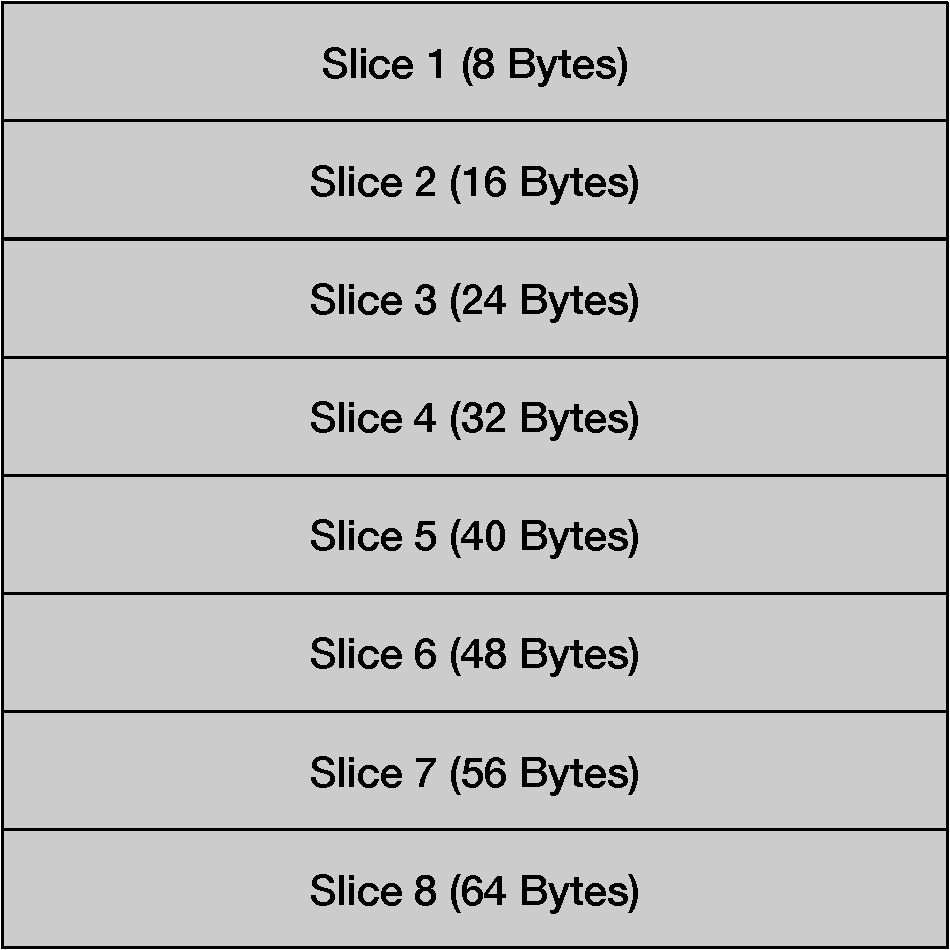
\includegraphics[width=\linewidth]{../figures/64-Byte-record.pdf}
  \caption{64-Byte Record. $8\times8$ byte slices, pre-emptible by responders} %Minimum record size is 64 Bytes; comprised of 8Bytes $\times$ 8 Slices, pre-emptable by the receiver}
\end{marginfigure}


%64-Byte-Record\footnote{Frames are variable Length in ATM -- return to original Manchester encoding where \texttt{record} is fixed size [ref] }

Frame size  of 64 Bytes. Follows a $log_2$ increase in slot size.  The first slot (Context) corresponds to the arrival of the first slice off the bits on the wire. Remaining slots follows a Hadamard multiple (1, 2, 4, or any multiple of 4 slices).

%\begin{enumerate}
%\item The protocol prioritizes information reliability and bandwidth allocation on a Neighbor-to-Neighbor (N2N), instead of an End-to-End (E2E) principle in conventional networks.
%\item Each pair of neighbor nodes is connected \emph{directly} to its neighbor and does not go through any other device or entity.  Advantages include:
%	\begin{itemize}
%	\item Security - Connections between nodes is private and near impossible to eavesdrop on without both parties being able to detect that.
%	\item Confinement - 
%	\item Temporal intimacy -- events on one side can be precisely correlated with events on the other side
%	\end{itemize}
%\item Processing of the packets is  organized in order to process information from the inside out
%	\begin{itemize}
%	\item LINK (Fast ULL computations in the Link itself. E.g. for ML/AI linear algebra operators)
%	\item CELL (the unit of network presence, whether or not it connects via PCIe bus to a host processor
%	\item TILE (Graph computations such as consensus (Paxos/Raft), including atomic cluster management
%	\item Local Topology Awareness beyond the 1-hop (3 x 3) tile.
%	\item	Remote Topology awareness of secure enclave boundaries and gateways to the IP world
%	\end{itemize}
%\end{enumerate}

\section{CONTEXT Processing : From the Inside Out}

\begin{description}
	\item [Slice 1] [8 Bytes LINK Context] Protocol  <RTL> 
	\item [Slice 2] [8 Bytes CELL Context]  Context]   <FSA>  <Linear Algebra>
	\item [Slices 3-4] [16 Bytes TILE Context] <State Machines><Petri-Nets>%<Interaction Nets>
	\item [Slices 5-8] [32-Bytes ] ULL App PAYLOAD> <Address Bridging> 
\end{description}

\subsection{Protocol hierarchy:  Four levels of Reversibility:}

\begin{itemize}
\item Context Slice Reversibility 
\item Shannon Information (Operand Zone A in Serdes)
\item Spekkens Knowledge (Operand Zone B  FPGAs, 2-3 clock cycles in)
\item Metcalfe Semantics (Operand Zone C in FPGA, 5-8 clock cycles in)
\end{itemize}

\section{Extended Addressing Modes for Legacy Compatibility}

To guarantee that no information is lost\footnote[][-50mm]{All distributed systems need transactions. Even applications that run on a single (multicore) machine need them.  If it runs in the cloud, it needs a transactional infrastructure underneath.}% to provide tenant provisioning \& isolation.}, 
the slots must be fixed size.  PCIe and CXL attempt to transfer 64 bytes minimum.  This makes the latency (occupation time on the wire) too long for ULL applications. Instead, we propose a minimum of the first slice (Protocol  -- Context).  Optional second slice  (Reliability/Recoverability). The rest is payload for local Ultra-Low-Latency (ULL) Transactions.

\begin{marginfigure}
%  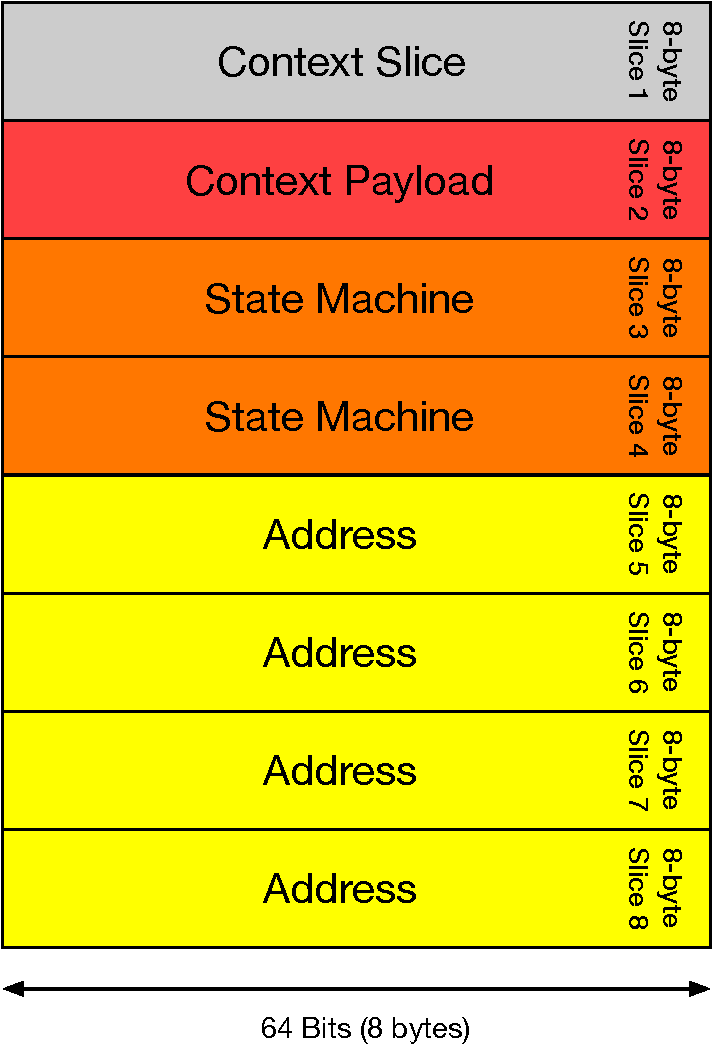
\includegraphics[width=\linewidth]{../Figures/addressing.pdf}
   \hspace{-18pt}    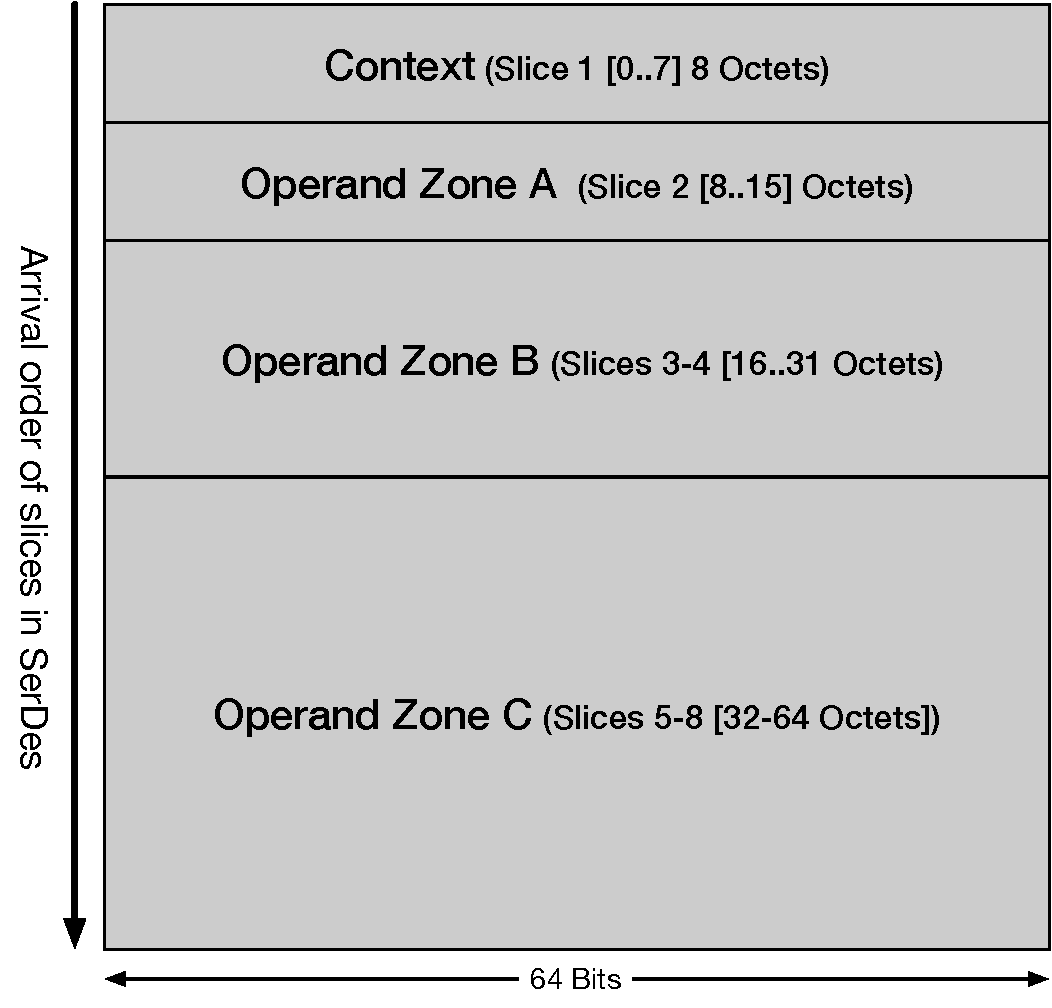
\includegraphics[width=1.12\linewidth]{../figures/slice-arrival.pdf}
  \caption{Slice Arrival order (Temporal  Intimacy Depth)}
\end{marginfigure}

\begin{description}
\item [Mode 1]- N2N Neighbor Self-Addressing
\item [Mode 2]- Ethernet MAC Addressing
\item [Mode 3]- 32-Bit IP Addressing
\item [Mode 4]- 128-Bit IP Addressing (Container virtual addresses?)
\item [Mode 5]- 10-Bit Cluster Addressing 12-bit VLAN Addressing.
\item [Modes 6..8]- Reserved
\item [Mode 7]- Reserved
\item [Mode 8]- Reserved
\end{description}

%\subfile{Protocol-byte} % This is already included in the main file.  THIS FILE HAS BEEN RENAMED ???

\newpage
\section{FLOW TRANSACTIONS}
%\marginnote{See \href{https://en.wikipedia.org/wiki/Ethernet_frame}{Ethernet Frame on Wikipedia}} 

\begin{marginfigure}
  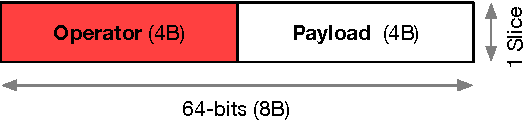
\includegraphics[width=\linewidth]{../figures/1-slice.pdf}
%    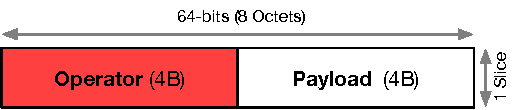
\includegraphics[width=\linewidth]{../../FIGURES/1Slice-Operator.pdf}
  \caption{1  Slice Flow Subtransaction}

\end{marginfigure}

ULL protocol designers play around with 32 bits as the minimum unit of transactional transfer, but experiments demonstrate the difficulty of making this consistently reliable i; the general consensus is that modern SerDes' work best with $\ge 64$ bit (8 Byte) slices/flits.
%Google Aquila, uses 16 byte flits.
Ethernet  has a minimum frame size of 64 bytes  (although only 42 bytes were available for the payload).

\begin{marginfigure}
%  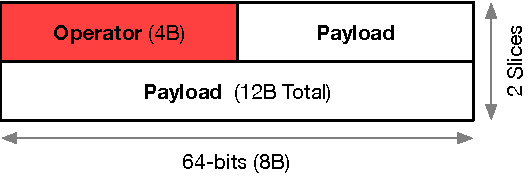
\includegraphics[width=\linewidth]{../Figures/2-slices.pdf}
    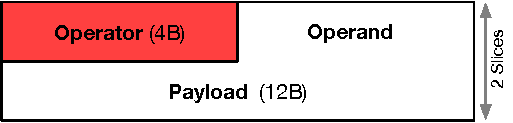
\includegraphics[width=\linewidth]{../figures/2-slice-operator.pdf}
  \caption{2 slice  Flow SubTransaction}% with 12B payload (operand)}
  \vspace{12pt}
\end{marginfigure}

We therefore choose a \emph{fixed} 64 Byte frame for the Shannon Slots, but make them \emph{pre-emptable} so that even the minimum size frame does not need to occupy space on the wire, increase latency, or FPGA processing steps, when the receiver has something more important it wishes to send (e.g. local status messages sent in the background can be pre-empted, giving way to a two phase commit (2PC) transaction).

\begin{marginfigure}
 % 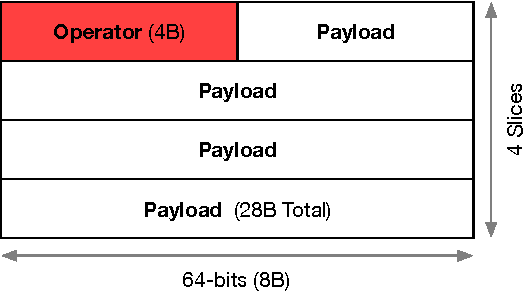
\includegraphics[width=\linewidth]{../Figures/4-slices.pdf}
      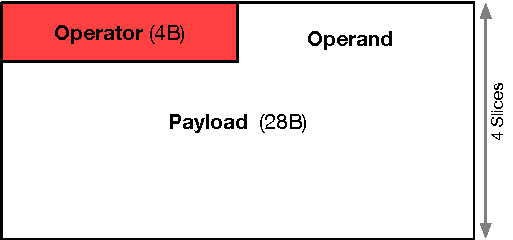
\includegraphics[width=\linewidth]{../figures/4-slice-operator.pdf}
  \caption{4 4 slice Flow SubTransaction with 28B payload (operand) \vspace{15pt}} % TODO Extraneous vspace. Need to eliminate
\end{marginfigure}

Some transactional systems are sensitive to making transactions reliable, but don't mind missing events, such as highly perishable market data.  We might call these one-phase commit (1PC) transactions. These can be made to flow at maximum line rate, even though each individual slice is being acknowledged. This is particularly important in HFT for example.

We therefore provide the following ``flow" transactions in the encoding scheme:

\begin{marginfigure}
%  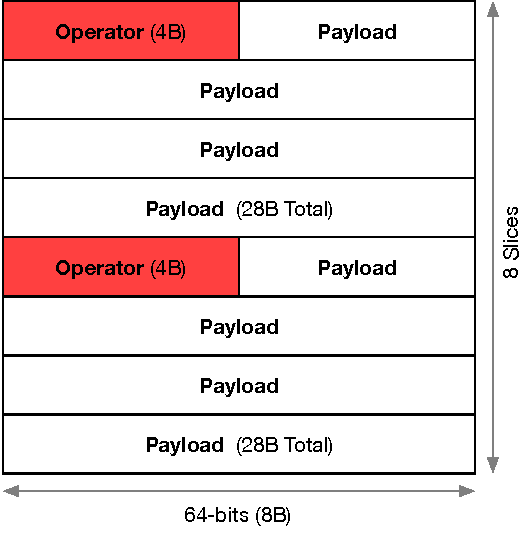
\includegraphics[width=\linewidth]{../Figures/dual-4-slices.pdf}
        \includegraphics[width=\linewidth]{../figures/8-slice-operator.pdf}
  \caption{1 $\times$ 8 slice Flow  Transaction with 60B payload}
\end{marginfigure}

% Reference Vortex by Ken Birman

\section{Back Propagation Encodings}
%* Modeled on the 2SVF

This encoding scheme (with slice acknowledgements), guarantees common knowledge in a flow of transactions, and their backpropagation packed into a single frame. Examples shown here include:


\begin{enumerate}
\item One Flow Transaction in with 4B payload in a single slice  (additional encoding in TX beats:
\begin{description} 
\item [\texttt{01}] I intend to send only one slice.
\item [\texttt{10}] I intend to send 2 slices, count down from there in replies
\item [\texttt{11}] I intend to send 4 slices, count down from there in replies
\end{description}
\begin{marginfigure}
  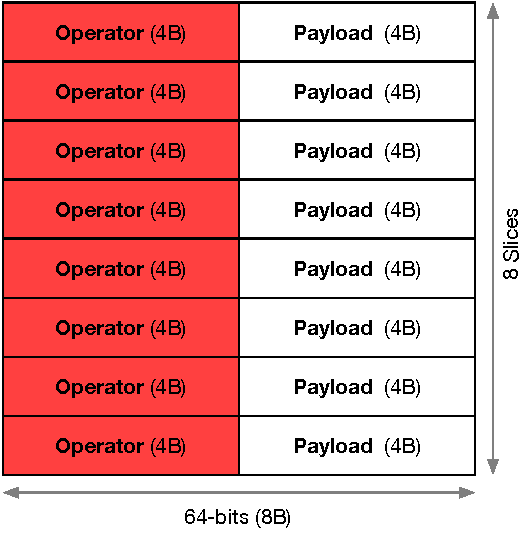
\includegraphics[width=\linewidth]{../figures/8-slices.pdf}
  \caption{8 independent Flow Transactions in a one frame}
\end{marginfigure}
\item One Two Slice  Flow Transaction context with 12B of Payload
\item One Four Slice  Flow Transaction context with 28B of Payload
\item Eight one-slice Flow Transactions context with 60B of Payload
\end{enumerate}


\clearpage
\section{Mixing and Matching Flow Transactions}

\subsection{Two 4 slice Flow Transactions}

\begin{marginfigure}
        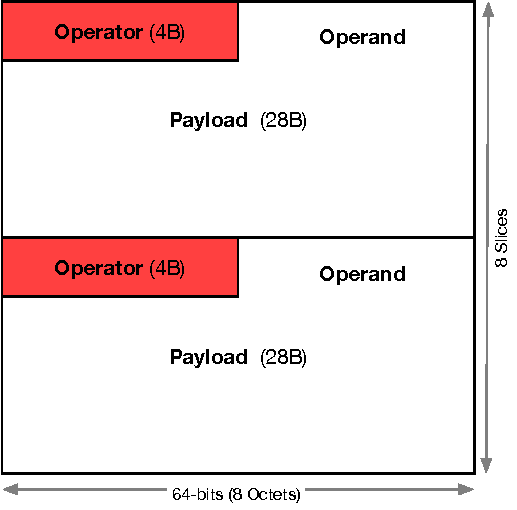
\includegraphics[width=\linewidth]{../figures/2-flow-subtransactions.pdf}
  \caption{2 $\times$ 4 slice Flow Transactions }
  \vspace{8pt}
\end{marginfigure}

You can also mix them in the same frame, but remember, they can only be used for One-Phase-Commit (1PC) in a single stream of transactions. This is because 1PC requires only one "round trip", whereas 2PC requires two round trips (although this scheme can be made to work for 2PC, and perhaps 4PC, but they have not yet been tested).

 
\subsection{Four  2 slice Flow Transactions}

\begin{marginfigure}
        \includegraphics[width=\linewidth]{../figures/4-flow-subtransactions.pdf}
  \caption{4 $\times$ 2 slice Flow Transactions}
    \vspace{8pt}
\end{marginfigure}

%\begin{marginfigure}
%        \includegraphics[width=\linewidth]{../../FIGURES/4-flow-subtransactions.pdf}
%  \caption{4 $\times$ 2 slice Flow Subtransaction}
%\end{marginfigure}
%

\subsection{Eight one-slice  Flow Transactions} 

%\begin{marginfigure} % This is already on the previous page
%        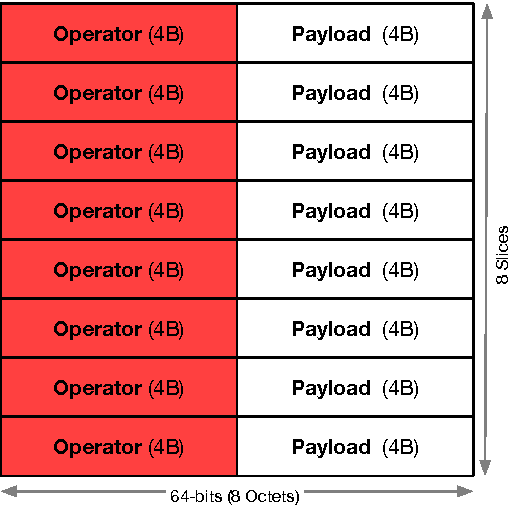
\includegraphics[width=\linewidth]{../../FIGURES/8-flow-subtransactions.pdf}
%  \caption{8 $\times$ 1 slice Flow Transactions}
%\end{marginfigure}



\subsection{Mixture of different  Flow Transactions} 

%[TESTING TO SEE IF FIGURES IN MARGIN SPREAD OUT CORRECTLY]

\begin{marginfigure}
        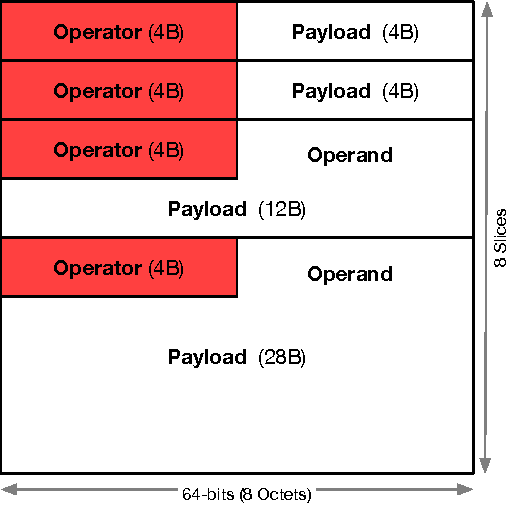
\includegraphics[width=\linewidth]{../figures/Mixed-1-2-4-slice-flowtransactions.pdf}
  \caption{One 8 slice Flow Sub Transaction with 60B payload}
    \vspace{8pt}
\end{marginfigure}

\section{Link Efficiency}

%------------------------------------------------
\begin{margintable}
\caption{Transaction efficiency by operator and operand size.}
\label{tab:txn-efficiency}

% Negative space shifts the table left;
% tune the value until the right edge no longer overflows.
\hspace*{-1.0em}% ← adjust (e.g., -0.5em, -1.5em, etc.)

\footnotesize            % (optional) make text slightly smaller
\setlength{\tabcolsep}{3pt} % (optional) tighten column padding
\hspace{-8pt}
\begin{tabular}{@{}r r r r@{}}
\toprule
Flows & Operator & Operand & Efficiency \\ \midrule
1 & 4 & 4  & 50\%   \\
1 & 4 & 12 & 75\%   \\
1 & 4 & 28 & 87.5\% \\
1 & 4 & 60 & 93.75\%\\
2 & 4 & 4  & 100\%  \\
2 & 4 & 12 & 150\%  \\
2 & 4 & 28 & 175\%  \\
2 & 4 & 60 & 187.5\%\\
4 & 4 & 4  & 200\%  \\
4 & 4 & 12 & 300\%  \\
4 & 4 & 28 & 350\%  \\
4 & 4 & 60 & 375\%  \\
8 & 4 & 4  & 400\%  \\
8 & 4 & 12 & 600\%  \\
8 & 4 & 28 & 700\%  \\
8 & 4 & 60 & 750\%  \\ \bottomrule
\end{tabular}
\end{margintable}
%------------------------------------------------



%\begin{marginfigure} % This is already on the previous page
%        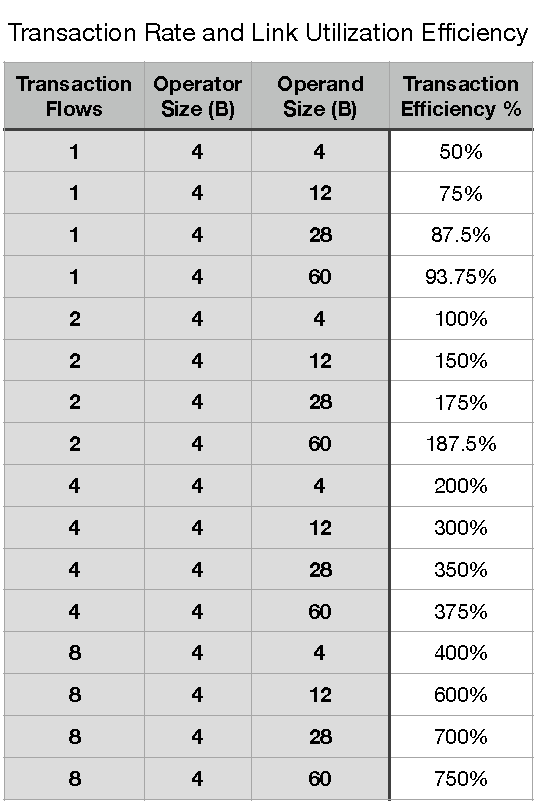
\includegraphics[width=0.92\linewidth]{../../FIGURES/Transaction-Rate.pdf}
%  \caption{Transaction Rate Calculations}
%    \vspace{8pt}
%\end{marginfigure}



%\begin{marginfigure}
%        \includegraphics[width=\linewidth]{../../FIGURES/8-slice-operator.pdf}
%  \caption{One 8 slice Flow Sub Transaction with 60B payload}
%\end{marginfigure}

%\subfile{Protocol-byte} % This is already included in the main file.

%
%\renewcommand{\bibfont}{\footnotesize}  % Footnote size for the whole bibliography
%\printbibliography

\newpage
\section{Virtual Channels}

The protocol provides Endpoints for Virtual Channels. The IPV6 Format has been proposed, but this would give the false impression that the outside world (Internet) and inside world (Transaction Fabrix)/ %tm].trademark doesn't work

\subfile{OPCODE-Byte}

\end{document}


